\documentclass[bachelor, comfort]{shtthesis}
\usepackage[fontsize=11.5pt]{fontsize}
\linespread{1.51}

% \pagestyle{MNNumberedWithLogo}

\usepackage{multirow}
\usepackage{float}
\usepackage{tablefootnote}
\usepackage{tikz}
\usepackage{amsmath}
\usepackage{graphicx}
\usepackage[list=off]{bicaption}
\captionsetup[figure][bi-second]{name=Figure}
\captionsetup[table][bi-second]{name=Table}

\renewcommand*{\vec}{\mathbf}

\shtsetup{
  title = {人脑的数量认知:\\数字表示与发展性计算障碍的探索},
  title* = {Numerical Cognition in the Human Brain: Exploring\\ Numerical Representation and Developmental Dyscalculia},
  keywords = {基本数量认知,三重编码模型,发展性计算障碍(DD),功能神经影像},
  keywords* = {Basic Numerical Cognition, Triple Code Model, Developmental Dyscalculia (DD), Functional Neuroimaging},
  date = {2024~年~06~月},
  date* = {06~/~2024},
  author = {王化雨},
  author* = {Huayu~Wang},
  author-id = {2020521003},
  entrance-year = {2020},
  institution = {生命科学与技术学院},
  institution* = {School~of~Life~Science~and~Technology},
  supervisor = {李远宁},
  supervisor* = {Yuanning~Li},
  discipline = {生物科学},
  discipline* = {Biological Science},
  bib-resource = {reference.bib},
}

\begin{document}


\maketitle

\pagestyle{RomanNumberedWithLogo}

\begin{abstract}
	基本数量认知是人类认知活动的基础。理解人脑处理和感知数字的神经机制对个人和社会的发展具有重要意义。个人层面,数量认知缺陷会影响就业和竞争力;国家层面,数学障碍会阻碍经济发展。

	三重编码模型是理解数量认知的主要框架,包括非符号和符号数字处理。非符号处理是直观的数量感知,符号处理将数学符号转换为数量。近年来的研究揭示了这些神经机制的关键点。

	发展性计算障碍(DD)是一种影响数量认知和算术技能的疾病,不涉及智力缺陷或资源不足。约5\%-7\%的人口受此影响,其神经机制仍有争议,但符号数字处理和近似数系统(ANS)功能异常是广泛认可的理论。

	本研究基于Fu Yu Kwok等人(2023)的工作,进行了细粒度的数量认知统计分析。结果显示,DD儿童与正常儿童在数字大小的脑激活上存在显著差异,揭示了数量认知的重要方面和潜在的干预目标。
\end{abstract}


\begin{abstract*}
	Basic numerical cognition is essential to human cognitive activities. Understanding the neural mechanisms of numerical processing and perception has significant implications for both individual and societal development. Individually, deficits in numerical cognition can affect employability and competitiveness, while nationally, mathematical disabilities can hinder economic growth.

	The Triple Code Model is a prominent framework for understanding numerical cognition, encompassing non-symbolic and symbolic number processing. Non-symbolic processing refers to intuitive quantity perception, while symbolic processing involves converting mathematical symbols into quantities. Recent studies have provided key insights into these neural mechanisms.

	Developmental dyscalculia (DD) is a disorder affecting numerical cognition and arithmetic skills, unrelated to general intellectual deficits or lack of resources. Affecting approximately 5\%-7\% of the population, DD's underlying neural mechanisms are still debated. However, impairment in symbolic number processing and the approximate number system (ANS) are widely recognized theories.

	This research builds on the work of Fu Yu Kwok et al. (2023) by conducting detailed analyses of numerical and quantity cognition. Our findings indicate significant differences in brain activation for numerical size between children with DD and their typically developing peers, highlighting crucial aspects of numerical cognition and potential targets for intervention.

\end{abstract*}

\makeindices

\clearpage
\pagestyle{MNNumberedWithLogo}


\chapter{引言} % (fold)
\label{chap:intro}

基本数量认知是现代人类思维活动的基石。更好的理解人脑处理数字信息、进行数字运算、以及对数量产生感受的神经机制有着巨大的意义。从个人角度而言,缺乏数量认知会大幅度影响人的就业情况和竞争力。有研究表明,基本数量认知和识字能力对于自我价值实现几乎同等重要\cite{num9}。从国家角度而言,数学障碍会导致严重的就业限制,影响经济发展\cite{num10}。

\section{基本数量认知}
目前,学术界对于数量认知的主流模型是三重编码模型\cite{num7}。该模型由\emph{Dehaene}等人在1993年提出\cite{tcm1},主要包括以下三个编码系统:
\begin{enumerate}
	\item \textbf{语义数量编码(Semantic Quantity Code)}:该编码系统与近似数系统(Approximate Number System, ANS)密切相关。它负责处理非符号数量信息,即不依赖语言或符号的数量感知。该系统在估计和比较数量时起主要作用,被认为是进化上较为原始的数量处理机制。
	\item \textbf{视觉阿拉伯数字编码(Visual Arabic Number Code)}:该编码系统处理符号化的数量信息,如阿拉伯数字。它负责将视觉输入的数字符号转换为数量信息,并在数学运算中发挥作用。
	\item \textbf{语言编码(Verbal Number Code)}:该编码系统与语言相关,处理以语言形式表达的数量信息(如“二十”)。它在语言基础上的数量处理和计算中起主要作用。
\end{enumerate}

该理论囊括了数量认知的方方面面,其中主要包括人脑对非符号数量和符号数字的感知使用的神经机制。非符号数量感知指的是人对不使用语言或数字的数量的直观感知能力。对数量的抽象感知能力是数字理解能力,数学运算能力发展的重要先决条件之一\cite{num11}。而符号数量感知指的是人将抽象的数学符号(如阿拉伯数字,自然语言中的数字等)转换成数量的能力。

近二十年来,有许多研究尝试明确这两个重要功能的神经机制,其中的一些重要结论改变了该领域对数量认知的理解。首先,近似数系统(approximate number system, ANS)是三重编码模型的核心\cite{num7}。它反映的是用直感去估计,区分物体数量的能力,为其他编码模式(自然语言,阿拉伯数字等)提供了语义基础。

许多研究表明,近似数系统与顶叶,尤其是右侧顶内沟(intraparietal sulcus, IPS)有较高的关联\cite{num14,num13}。并且,编码数字响应的神经元遵循韦伯-费希纳定律\cite{num16,num15}。

\begin{figure}[ht]
	\centering
	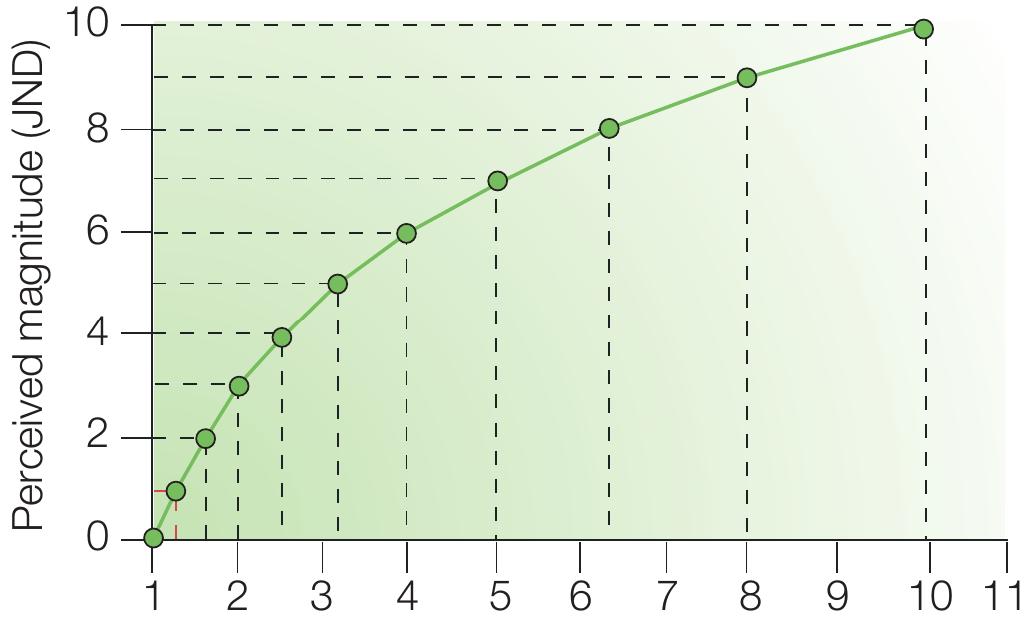
\includegraphics[width=0.60\linewidth]{figures/weber.png}
	\caption{\label{fig:weber} 感知刺激强度与实际刺激强度关系,图引用于\cite{num15}}
\end{figure}


也就是说,随着刺激数量的变大,区域的总神经相应将以对数规律上升。这个结论在非灵长类动物的单神经元电信号记录以及人的功能核磁共振实验中都得到了应证\cite{num18,num17}。另一个非符号感知的重要系统是物体追踪系统。这个神经系统主要和计数有关,负责区分和追踪不同的物体。该系统主要和顶叶皮层,视觉皮层,和颞顶交界处(temporoparietal junction, TPJ)有关\cite{num20,num19}。符号感知则更多涉及与视觉和注意力相关的脑区。数字符号在枕叶皮层被处理,随后在IPS映射为数量\cite{num21}。有趣的是,符号感知的神经响应会随着年龄、数学技能、教育水平改变。随着数学水平或熟悉程度的提升,顶叶,下部前额叶(inferior frontal cortex),和枕叶的激活会上升\cite{core95,core14,core94,core30};而前额叶,前扣带回(anterior cingulate gyrus)的激活会下降\cite{core95,core87,core30}。这可能意味着随着数学能力的上升,顶叶和枕叶的自体化上升\cite{num22},执行这些任务时所需的注意力减少。另一个对于人脑理解符号数字的重要维度是计数的技能。孩童用手指来数数似乎是稀松平常的事情,但是事实上,习得计数技能对于孩童掌握基本数字运算,理解符号数量的顺序关系都有着很大的作用\cite{num23}。更准确地说,计数代表着通过建立物体与符号数字(或者其他可代表数量的物体,如手指)之间的一一对应,随后迭代的共同遍历物体和符号数字,以至于物体迭代完毕之后所对应的符号数字就代表那堆物品的数量。这种知识被称为势原则(cardinal principle)\cite{num24}。

研究表明,孩童习得势原则之后大大加速了符号数字的学习\cite{num25}。以上是目前学界对基本数量认知的一些重要结论。

\section{发展性计算障碍}
根据世界卫生组织(world health organization, WHO)的现行定义,发展性计算障碍(developmental dyscalculia, DD)是一种影响数字认知和算术技能学习的发育性疾病。其通常表现为难以处理和加工数字,计算准确性差等。这些困难并不是智力发展问题、 感官系统损伤、精神或神经疾病、学习资源缺乏所导致\cite{who}。目前,全球大约5\%-7\%的人群患有计算障碍\cite{num29,num28}。对于发育性计算障碍的发病机制和神经基础,学界有诸多理论解释,但未有统一定论。其中有两个理论受到学界的广泛认可,其一是处理符号数字能力受损\cite{num30}。由于在患有DD的孩童中,符号数字能力受损较为广泛,所以有些研究认为该差异可以被用于DD的诊断\cite{num31}。另一个是处理或表达数量的能力受损(即ANS功能异常)\cite{num32}。虽然上述研究表明,这些系统的非常规激活与DD的发病强相关,但这些功能异常与DD的因果关系尚不明确。正是因为DD的发病与这些核心系统的受损有强烈的联系,研究DD人群与正常人群的神经表达差异成为了研究基本数量认知的绝佳切入点。


\section{使用功能核磁共振研究大脑活动}
功能性磁共振成像(functional Magnetic Resonance Imaging, fMRI)是一种强大的神经影像学技术,可以用于研究大脑活动。fMRI通过检测血氧水平依赖(blood oxygen level dependent, BOLD)信号来间接测量脑活动。当大脑区域在执行某个任务时,其血流量会增加,导致局部含氧血红蛋白浓度上升,BOLD信号由此产生\cite{bold1}。使用fMRI研究神经活动是一把双刃剑。其中最显著的优点包括:

\begin{enumerate}
	\item 极高的空间分辨率
	\item 非侵入式
	\item 全脑记录
\end{enumerate}

因为这些优点,fMRI尤其易被研究者接纳。但是,由于fMRI本身的性质,使用它来研究神经活动也有几个限制:

\begin{enumerate}
	\item 低时间分辨率
	\item BOLD信号无法直接反映神经活动
	\item 高噪声
\end{enumerate}

在数量认知的研究中,fMRI被广泛用于探索不同脑区在处理数量信息时的功能。通过任务设计和数据分析,研究者可以识别与数量认知相关的脑区,理解其在符号和非符号数量处理中的作用。并且,TCM模型已经在fMRI模态下得到了验证\cite{bold2}。这些研究不仅深化了我们对数量认知的理解,也为发展性计算障碍的神经机制研究提供了重要线索。利用fMRI,我们可以比较被试在处理阿拉伯数字和点阵数量时的脑活动模式,探索DD的神经机制。


\section{研究内容}
近年来,许多使用功能神经影像的方法研究DD神经机制的工作都存在样本量少,结果无法复现的问题\cite{num33}。而\emph{Fu Yu Kwok}等人在2023年发表的工作是迄今为止规模最大的\cite{num1}。本研究在此工作的基础上,针对具体数字与数量认知进行粒度更细的统计研究和探索。本研究探索了单个数字,奇偶对比,数字大小对比在DD孩童与正常孩童中的激活情况。数据表明,患有DD的孩童与正常孩童相比,对于数字大小有差异相应的脑区激活情况存在显著差异。其他刺激和对比均无显著差异。

% chapter  (end)

\chapter{实验方法与材料} % (fold)
\section{数据集概况和被试分布}
为了使用高精度的神经响应数据研究数字在人脑中的表示,我们选择了\emph{Fu Yu Kwok}等人发表的公开数据集进行实验\cite{num1},主要研究内容是发展性数学技能障碍(Developmental dyscalculia, DD)是否与非典型的大脑激活有关。该研究使用了3T功能核磁共振对68个新加坡的小学阶段参与者(平均年龄 = 8.95岁,标准差 = 0.34岁;男性30名)完成了扫描。参与者被分为了两组: 发展性计算障碍组(DD)和典型发展对照组(TA)。DD组包括30名儿童,这些儿童要么参与了数学学习支持(LSM)干预计划,要么在一年级时的标准化数学测试中成绩处于后10\%。这两组儿童在任何时间点的数学评估中均无显著差异。TA组包括38名儿童,他们在一年级时的数学测试得分高于25百分位,并在年龄、性别、种族、民族和社会经济地位等方面与DD组儿童匹配。

\section{实验任务}
该研究使用了三个实验任务:算术任务、匹配任务和视觉空间工作记忆任务。由于本文聚焦于研究符号数字与非符号数字在大脑中的初级语义表示,我们的研究仅使用匹配任务的数据。具体任务设计如下:

每个参与者都完成了两轮试验,每轮试验包括三种条件的六个试验块(总共36个试验),每个试验块前都有一个带有示例刺激的提示,一个初始的注视块(6500毫秒)和一个结束的注视块(12000毫秒)。每个块包括一个条件的六个试验,带有平均1500毫秒的抖动试验间隔(ITI)。匹配任务的流程图如图\ref{fig:trial}所示

\begin{figure}[ht]
	\centering
	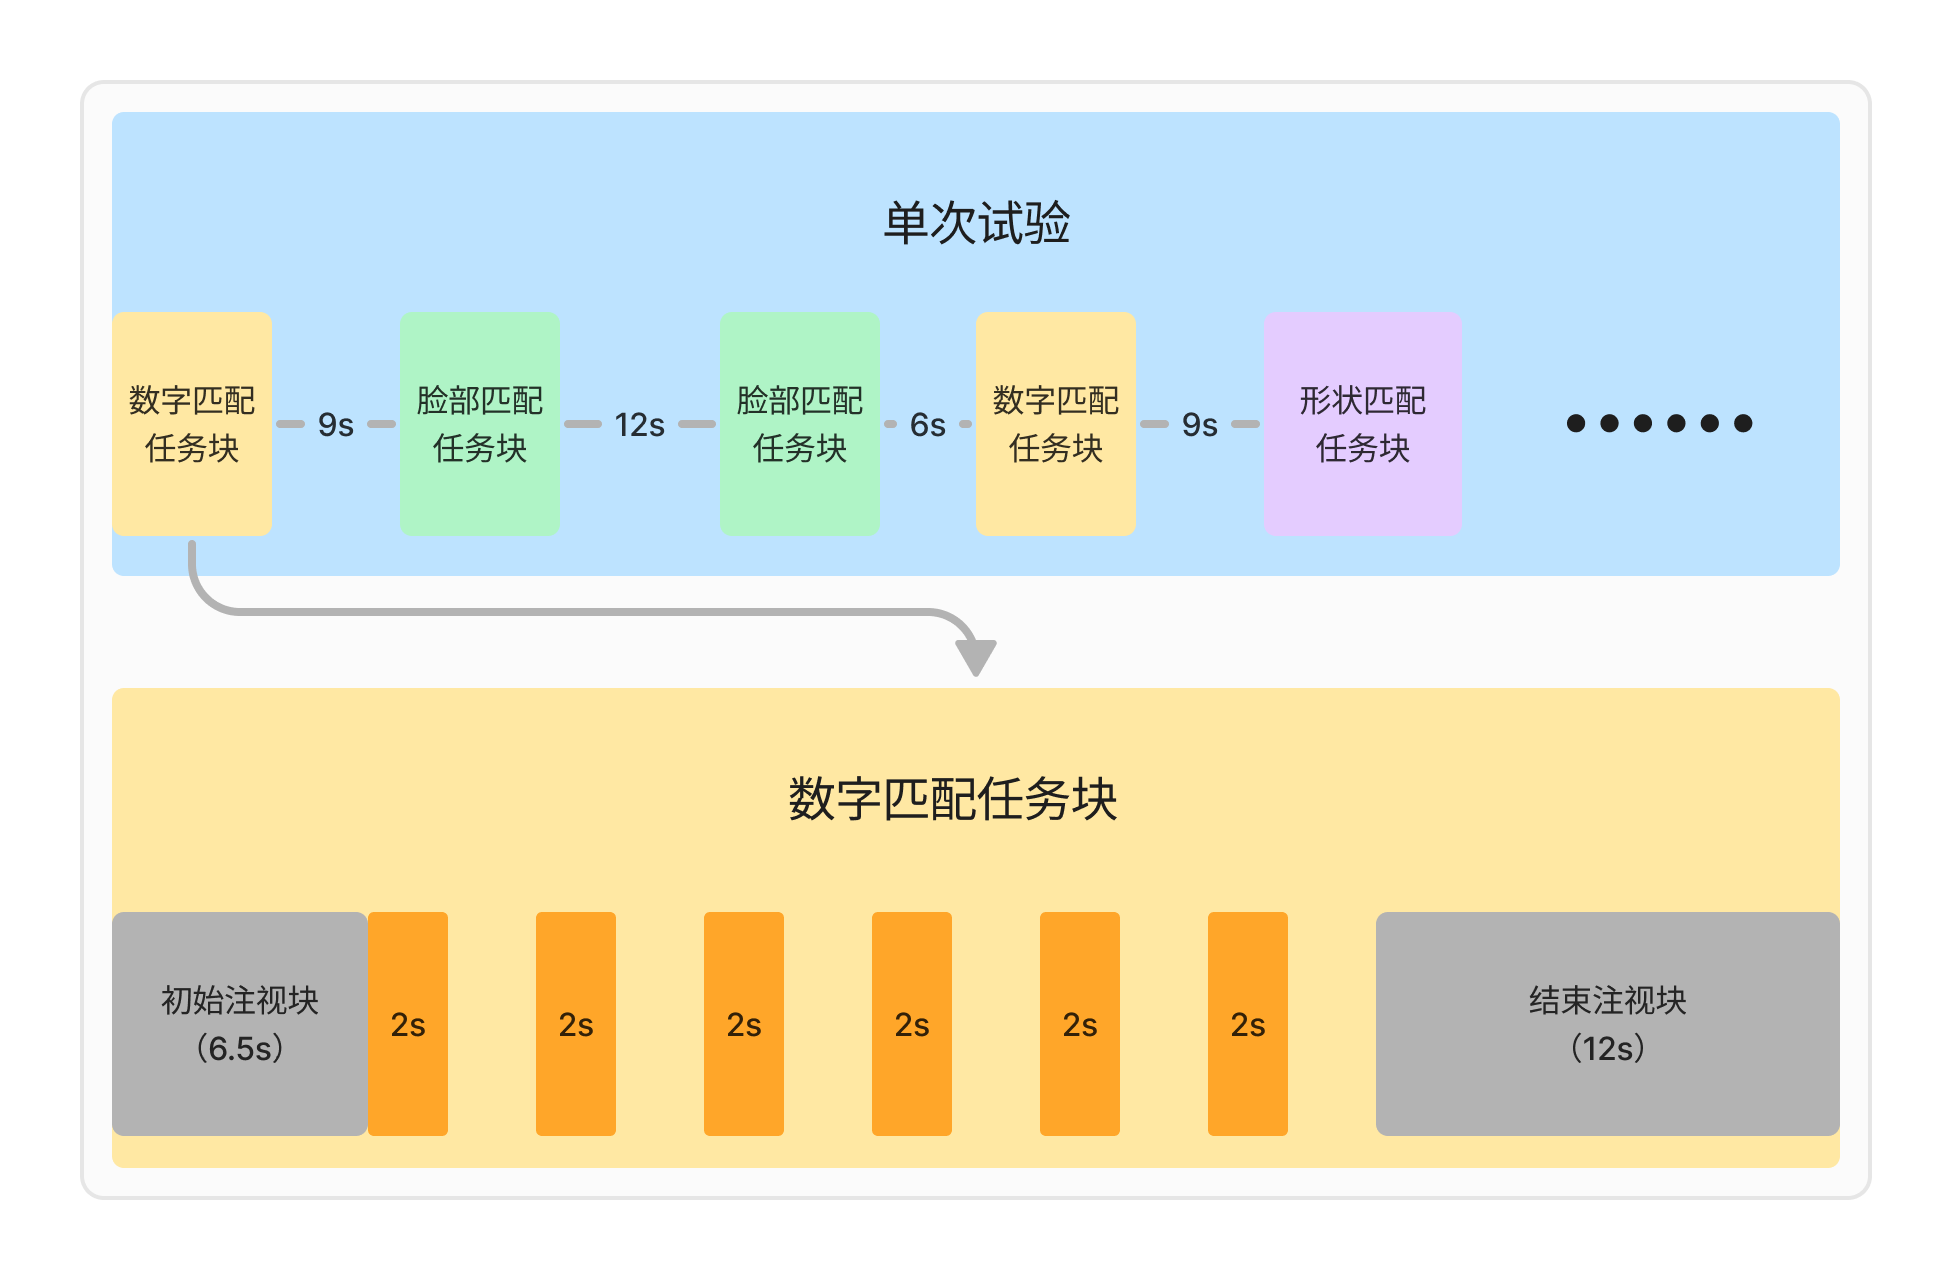
\includegraphics[width=1.0\linewidth]{figures/trial.png}
	\caption{\label{fig:trial} 匹配任务的流程图。块间休息时长平均为9s,每块包含6个测试。}
\end{figure}

其中三种实验条件分别为:数字条件、形状条件、脸部匹配。每个条件中,参与者同时被呈现左右两个刺激(数字条件中为一个数字符号和一组点、形状条件中为两个形状、脸部匹配条件中为两个正面的亚洲面孔),并被要求判断这两个刺激是否相同,每个刺激呈现2000毫秒。对于其他实验细节与设计,请参考该工作\cite{num1},本文不再赘述。

在后续实验中,形状匹配和脸部匹配条件将作为隐含基线,用来对比数字匹配任务相关的激活。值得一提的是,该工作中总是使用形状匹配或者脸部匹配条件作为基线。由于我们将数字匹配条件进一步细分,以下的实验中,我们不将实验条件和具体的形状或脸部匹配人物作对比,而仅仅使用隐含基线作为实验基准。

值得一提的是,该工作中对DD和TA的组别分析结果几乎都对$\mathbf{H}_0$(两组无明显差异)有强支持。这使得作者得出了DD和TA组无明显神经响应差异的结论。但是在匹配任务中,数字条件>形状条件的对比分析找出了三个显著的激活簇,而其余99.6\%的体素都显示$\mathbf{H}_0$。在本实验中,我们将在具体数字条件刺激的层面对这个结论进行分析。在对于人脑数字表示的研究中,我们可以认为DD和TA组无显著差异,将其归为一个组别进行研究。

\section{数据预处理和分析方法}
我们对于数据的处理和分析使用fMRIPrep\cite{num2},NLTools\cite{nltools},Nipy\cite{nipy},Nilearn\cite{nilearn}等工具进行。首先,我们使用标准的fMRIPrep管线对数据进行预处理,并使用NLTools对单被试的每个体素构建广义线性模型(general linear model, GLM)。随后,我们对每个本文关注的对比条件(单个数字刺激与基线对比、奇偶对比、大小对比)进行了组内统计检验(单采样t检验)。对与组内统计检验结果较为显著的对比,我们进行了组间统计检验(双采样t检验)。最后,我们还尝试使用多体素模式分析对组间差异在多体素层面的研究并进行了显著性检验。总体实验管线如图\ref{fig:pipeline}所示。

\begin{figure}[ht]
	\centering
	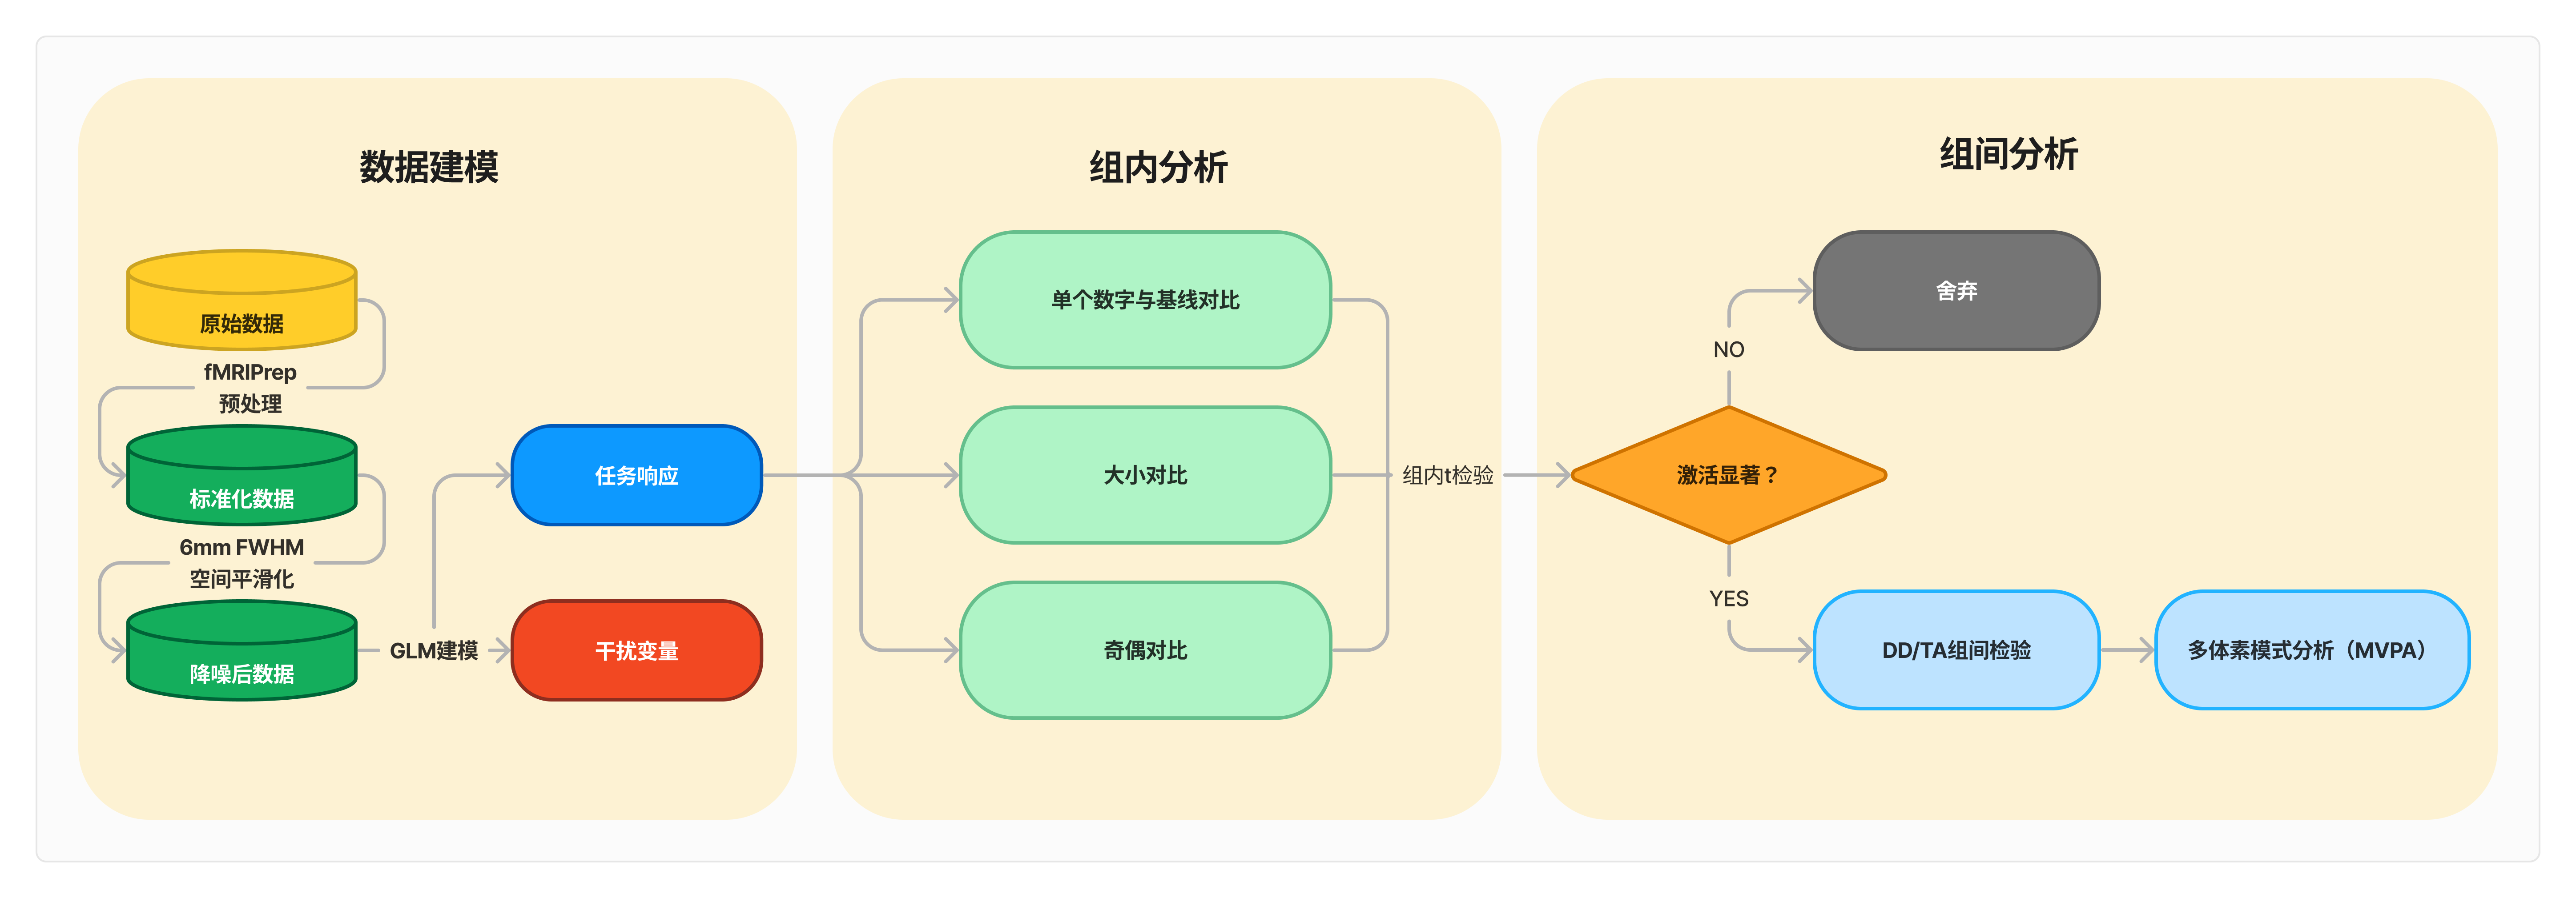
\includegraphics[width=1.0\linewidth]{figures/pipeline.png}
	\caption{\label{fig:pipeline} 数据处理与分析管线图 }
\end{figure}


\subsection{数据预处理}
我们使用发布在Openneuro\footnote{\url{https://openneuro.org/datasets/ds004791/versions/1.0.0}}的公开数据进行研究。该数据集已经经过去面处理。我们使用fMRIPrep\cite{num2}对所有数据进行预处理。结构图像经过不均匀性校正并标准化至MNI标准空间(MNI-ICBM 152)。功能图像进行了切片时间校正,估算了头部运动参数,并与T1加权参考图像进行配准。BOLD时间序列也标准化至MNI标准空间,然后经过6毫米全宽半高(full width at half maximum, FWHM)高斯核的空间平滑处理。每一个被试的具体处理参数和细节可根据要求提供。

\subsection{单被试GLM建模}
影响fMRI数据的因素是多种多样的,并非仅有实验刺激的影响。首先,由于BOLD信号的特性,被试接受实验刺激后的响应情况并非线性。每张fMRI影像都将被前几个实验任务所影响。其次,fMRI数据还会受到许多干扰因素的影响。被试的头部移动,fMRI仪的线性或非线性漂移,快慢振荡以及其他噪声都会对fMRI记录产生影响。因此,分离这些干扰变量的影响因素是很有必要的。为此,我们使用GLM对每个被试的每次测试的单个体素进行建模。

GLM是对线性回归模型的拓展,它允许目标变量具有任意的分布。通过引入链接函数(link function),GLM可以将线性预测器(linear predictor)与目标变量的期望值联系起来,从而适应不同类型的数据。常见的GLM包括线性回归、逻辑回归和泊松回归等,它们分别处理不同分布的数据。在fMRI数据分析中,GLM被广泛应用于分析脑活动和实验条件之间的关系。通过GLM,我们可以构建设计矩阵(design matrix),其中包括实验条件、头部运动参数和其他潜在的干扰因素。然后,我们对每个体素进行时间序列分析,将BOLD信号与设计矩阵中的各个预测变量进行拟合。这个过程中,GLM可以帮助我们分离出实验刺激对BOLD信号的影响,减小其他干扰因素的影响。

在GLM中,我们使用以下数学形式来表示模型:

\[ \mathbf{Y} = \mathbf{X} \boldsymbol{\beta} + \boldsymbol{\epsilon} \]

其中:

\begin{enumerate}
	\item \(\mathbf{Y}\) 是观测到的响应变量的向量,长度为 \(n\)(观测次数)。
	\item \(\mathbf{X}\) 是设计矩阵(design matrix),维度为 \(n \times p\),其中 \(n\) 是观测次数,\(p\) 是回归变量的数量。设计矩阵的每一列代表一个回归变量,例如实验条件、头部运动参数等。
	\item \(\boldsymbol{\beta}\) 是回归系数的向量,长度为 \(p\)。这些系数表示每个回归变量对响应变量的贡献。
	\item \(\boldsymbol{\epsilon}\) 是误差项的向量,长度为 \(n\),表示模型未能解释的部分。
\end{enumerate}


更具体地,我们可以展开设计矩阵和回归系数向量来表示:

\[ \begin{bmatrix}
		Y_1    \\
		Y_2    \\
		\vdots \\
		Y_n
	\end{bmatrix} = \begin{bmatrix}
		X_{11} & X_{12} & \cdots & X_{1p} \\
		X_{21} & X_{22} & \cdots & X_{2p} \\
		\vdots & \vdots & \ddots & \vdots \\
		X_{n1} & X_{n2} & \cdots & X_{np}
	\end{bmatrix} \cdot \begin{bmatrix}
		\beta_1 \\
		\beta_2 \\
		\vdots  \\
		\beta_p
	\end{bmatrix} + \begin{bmatrix}
		\epsilon_1 \\
		\epsilon_2 \\
		\vdots     \\
		\epsilon_n
	\end{bmatrix} \]

在这个模型中,\(\mathbf{X}\) 的每一列代表一个特定的回归变量(例如一个实验条件或一个干扰因素),而每一行对应一个观测值。回归系数 \(\boldsymbol{\beta}\) 表示每个回归变量对响应变量 \(\mathbf{Y}\) 的影响大小。误差项 \(\boldsymbol{\epsilon}\) 则表示不可预测的噪声或误差。

通过拟合GLM模型,我们可以估计回归系数 \(\boldsymbol{\beta}\),从而理解每个回归变量对响应变量的贡献。这对于分析fMRI数据中的不同实验条件对脑活动的影响尤为重要。

我们使用NLTools\cite{nltools},Nipy\cite{nipy},Nilearn\cite{nilearn}等工具对每个被试的匹配任务响应进行了GLM建模。对每个条件下每个试验的预期BOLD信号使用双伽马血氧动力学响应函数(hemodynamic response function, HRF)进行建模。为了研究与每个数字刺激(1-9)的响应,在GLM的建模过程中,我们保留形状、脸部匹配条件的回归变量,而将数字条件拆分。对于每个被试观看的左,右刺激所对应的数字分别建模,得到对应左,右9个数字共18个回归变量。其中,每个数字刺激均有阿拉伯数字和点阵两种刺激形式。我们将这两种形式归为一类进行回归。为了排除干扰变量的影响,我们还加入了离散余弦变换(discrete cosine transformation, DCT),二阶线性趋势,头部运动,和尖峰所对应的回归变量。最终通过回归,得到每个回归变量(数字1-9的左右刺激、形状匹配、脸部匹配、干扰变量)所对应的\(\boldsymbol{\beta}\)值。

%一个设计矩阵(\(\mathbf{X}\))的例子如图所示。


通过这些处理步骤,我们能够获得更为可靠和一致的神经影像数据,为后续的分析奠定坚实的基础。我们使用的所有分析代码发布于GitHub\footnote{\url{https://github.com/PlaneTraveller/numbers-in-brain}}。

\subsection{单变量统计检验}
为了检验我们所感兴趣的任务刺激下的神经响应是否在人群中有显著性,我们在单体素层面进行t检验。单采样t检验用于检验一个样本均值是否显著不同与一个已知的总体均值(通常为零),而双采样t检验用于检验两个样本的均值是否显著不同。一般而言,我们将零假设$\mathbf{H}_{0}$设置为样本均值为0的情况,而当零假设成立的概率($p$)值足够低时,我们认为该体素的响应是显著的。数学上,$p$值由t统计量对应的t分布上的累积分布函数(CDF)所计算。

\begin{enumerate}
	\item \textbf{单采样t检验}\\
	      假设我们有一个样本数据 \(\mathbf{X} = \{X_1, X_2, \ldots, X_n\}\),其均值为 \(\bar{X}\),标准差为 \(s\),样本大小为 \(n\),已知总体均值为 \(\mu_0\),则单采样t检验的t统计量计算公式为:
	      \[
		      t = \frac{\bar{X} - \mu_0}{\frac{s}{\sqrt{n}}}
	      \]

	\item \textbf{双采样t检验}\\
	      假设我们有两个独立样本 \(\mathbf{X}_1 = \{X_{11}, X_{12}, \ldots, X_{1n_1}\}\) 和 \(\mathbf{X}_2 = \{X_{21}, X_{22}, \ldots, X_{2n_2}\}\),它们的均值分别为 \(\bar{X}_1\) 和 \(\bar{X}_2\),标准差分别为 \(s_1\) 和 \(s_2\),样本大小分别为 \(n_1\) 和 \(n_2\)。双采样t检验的t统计量计算公式为:
	      \[
		      t = \frac{\bar{X}_1 - \bar{X}_2}{\sqrt{\frac{s_1^2}{n_1} + \frac{s_2^2}{n_2}}}
	      \]
\end{enumerate}


\subsection{多体素模式分析}
以上介绍的分析方法都属于单变量分析。在神经信号处理的语境中,这指的是我们将单独的体素作为研究对象,而不考虑体素与体素之间的相关性。很多时候,针对单体素的分析是不够的。我们希望分析激活簇甚至脑区与实验刺激的关系。为了达到这一目的,我们需要进行多体素模式分析(multivoxel pattern analysis, MVPA)。具体来说,我们使用监督学习的方法,训练模型使用我们挑选的体素信息,反过来预测我们关心的结果变量。

\[\text{outcome}=\sum_{i}^{n}\beta_{i}\cdot \text{voxel}_{i}+\epsilon\]

在MVPA中,支持向量机(Support Vector Machine, SVM)是常用的分类器之一。SVM是一种强大的监督学习方法,广泛应用于分类和回归任务中。它通过找到一个最优的超平面,将数据分为不同的类别,从而实现分类的目的。在本文中,我们选取特征体素,并在这些体素上训练SVM分类器进行二分类,从而研究我们选择的这些体素总体上是否能反应组间差异。此外,为了验证分类的显著性,我们还采用了置换检验的方法来计算得到该分类结果的概率。其原理是重复地随机置换样本与标签的对应关系,从而构造出检验量的经验分布,得到分类结果的统计显著性。



\chapter{实验结果与分析} % (fold)
\section{对单个数字的响应}
\subsection{组内基准对比}
首先,为了大致观察每个数量刺激是否在人群中有显著激活,我们绘制了每个数量刺激(1-9)在全体参与者(TA+DD)中的激活图。在本实验中,我们将形状匹配条件的响应作为基线。具体来说,在每轮实验中,对于每个数量刺激,我们将每个被试的左右刺激响应进行平均,随后减去形状匹配任务的响应——即数量>形状对比。随后对每个被试每轮实验中的数量>形状对比进行单采样t检验,绘制出响应显著的区域(FDR修正,$q<0.05$)。对应每个数量刺激的激活图如图\ref{fig:nums_activation}所示。

\begin{figure}[hp]
	\centering
	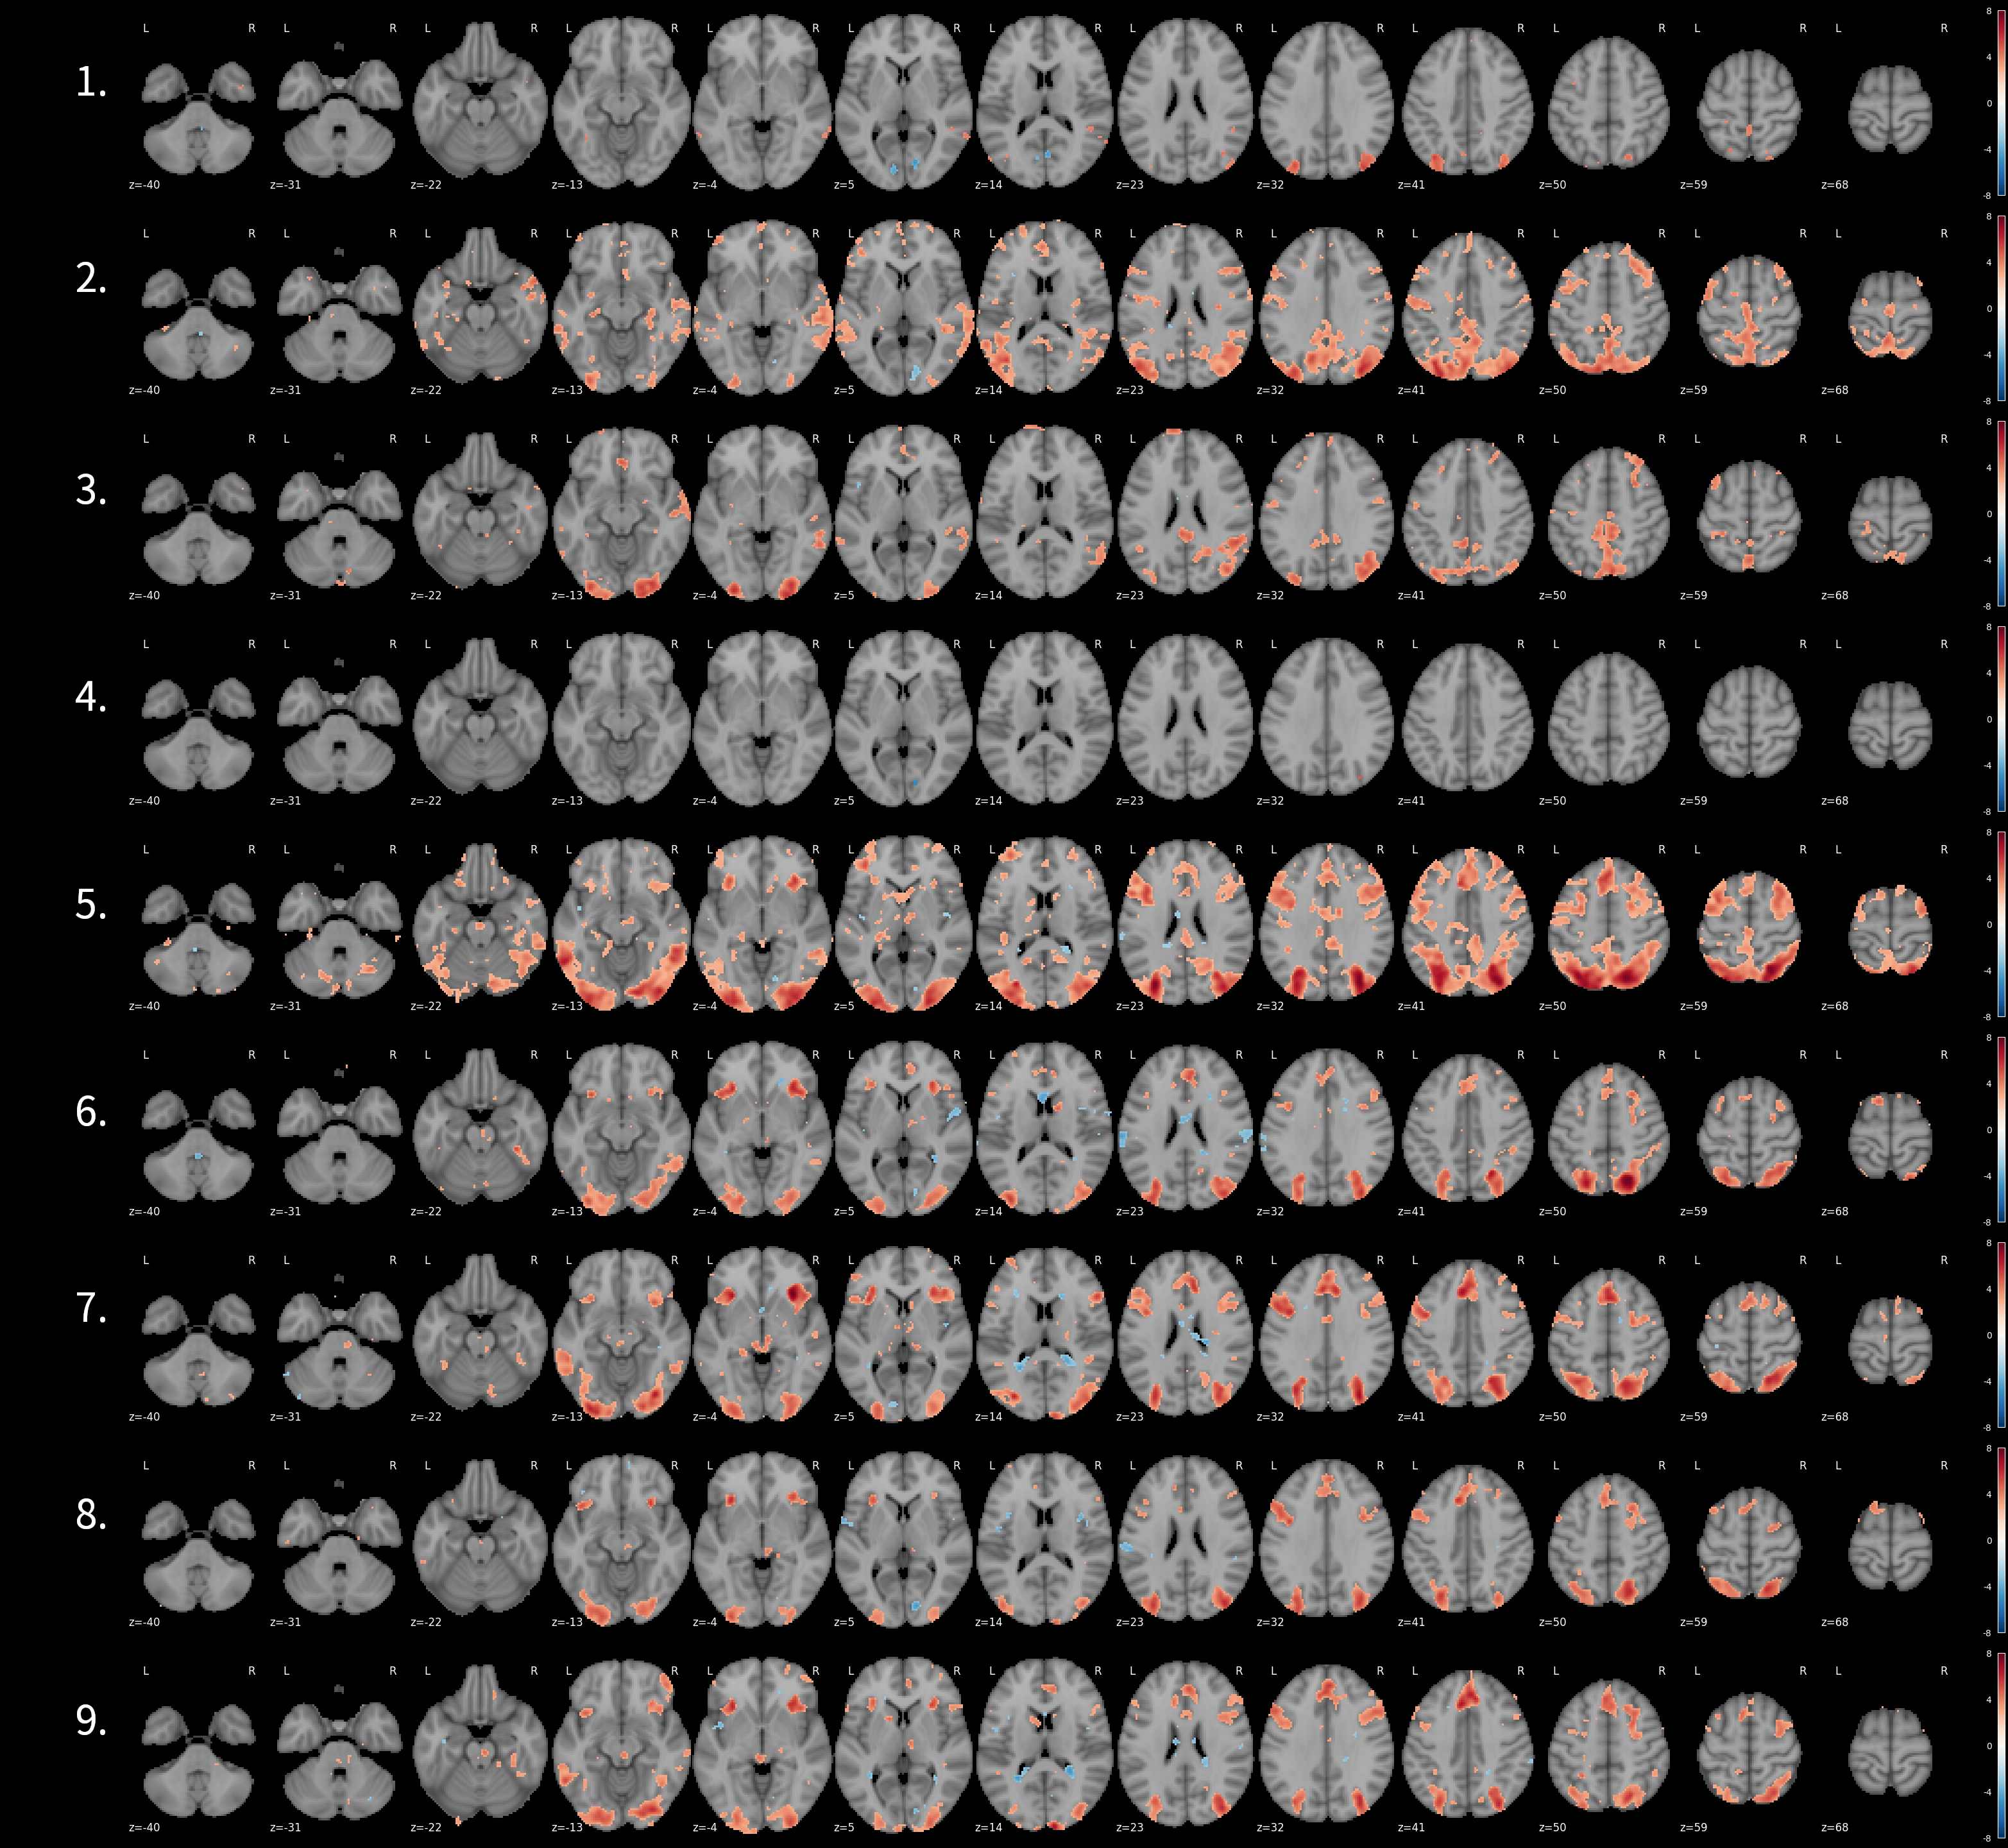
\includegraphics[width=0.95\textwidth]{figures/1_nums_activation_map.png}
	\caption{\label{fig:nums_activation} 每个数量刺激(从上到下依次为数量1-9)在全体参与者(TA+DD)中的单采样t检验t值(FDR修正,$q<0.05$),$-8<t<8$}
\end{figure}

除了数量4以外,其他数量均有显著激活。在大部分数量中观察到枕叶皮层激活,但有趣的是,较小的数量中(1, 2, 3, 4)没有显著的前额叶,前扣带皮层,前岛叶激活,而较大的数量中(5, 6, 7, 8, 9)有显著激活。此外,在数量2, 3, 5中观察到显著的后扣带皮层激活。这表明,单个数量在人脑中有激活,并且存在数量与数量间的激活差异。

\subsection{组间比较}
随后,我们探索了每个数量 刺激在DD与TA组中的激活差异。对于每个数量刺激,我们在两个组中进行了基于GLM回归的双采样t检验。其设计矩阵采用了对比设计,即一个截距回归器(全部为1的列)和一个对比回归器(对应TA组的行为-1,对应DD组的行为1)。相较于组设计,对比设计可以更好地将两组的差异激活分离出来。每个数量对比的激活图如图\ref{fig:number_contrast}所示。

\begin{figure}[hp]
	\centering
	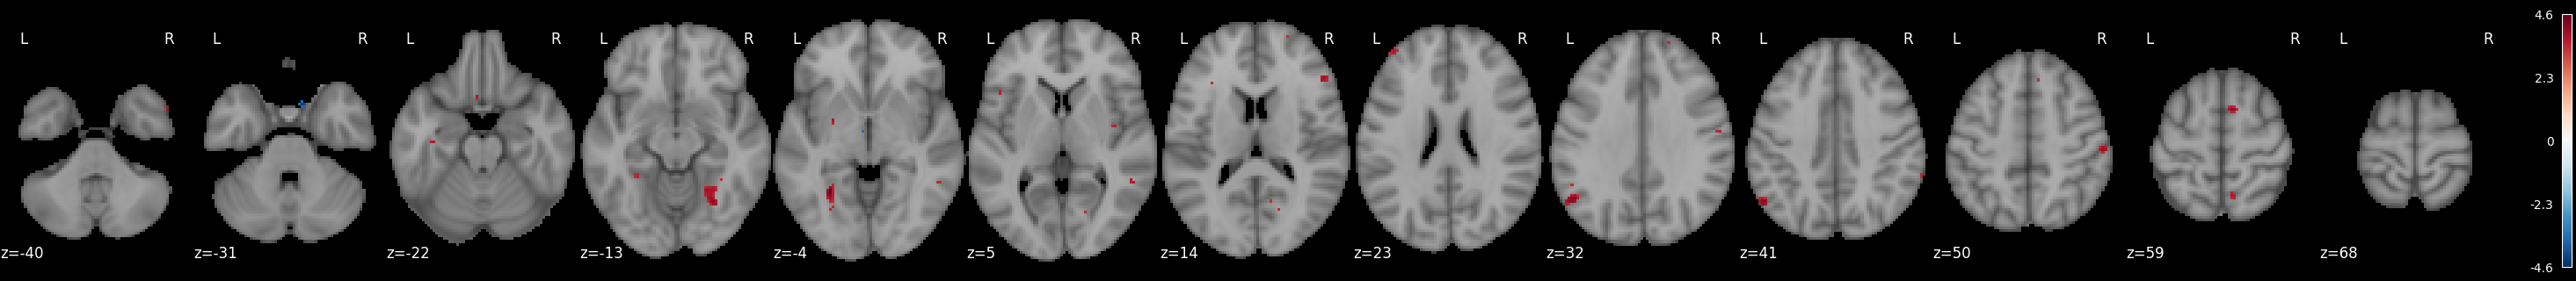
\includegraphics[width=0.95\textwidth]{figures/2_number_contrast.png}
	\caption{\label{fig:number_contrast} 数量1刺激的双采样t检验t值($p<0.001$, uncorrected)}
\end{figure}

其中仅有数量1刺激在DD与TA组中有显著的差异激活。数量1的差异激活主要在前额叶,后扣带皮层,枕上回,以及右侧与海马旁回相邻的V2区域。除了数量1之外,DD与TA组间并无显著激活差异。

值得一提的是,数量7刺激也显示了显著的差异激活,但是激活区域为右侧运动皮层。由于实验任务涉及使用右手按下按钮,这样的差异激活很可能是由于DD组实际按下按钮的次数更少所导致的,并且原工作中也检测到了类似的激活。此激活属于误差。

然而,分析每个数量的组间激活差异并不能指向DD和TA组处理数量信息的功能性差异。为了解决这个问题,我们天然的提出了两种假设:

\begin{enumerate}
	\item DD和TA组在处理奇偶数量时有显著的神经响应差异。
	\item DD和TA组在处理大小数量时有显著的神经相应差异。
\end{enumerate}

随后,我们为这两种假设分别设计了单独被试对比,然后在对比的基础上进行了组内单采样t检验、组间双采样t检验。实验表明,在奇偶对比(c = [1, -1, 1, -1, 1, -1, 1, -1, 1])下,无论是全体参与者(TA+DD),还是对照组(TA),或计算障碍(DD)组内t检验都显示零假设成立。该结果表明,在孩童中并无可以被当前实验条件探测到的奇偶响应差异。

\section{对大小数量的差异响应}
为了表征体素对于大小数量的差异响应,我们在对比的设计中使得在数轴上距离越远的数量的响应差异也更大(c = [-4, -3, -2, -1, 0, 1, 2, 3, 4])。这样的设计有助于放大数量大小的差异,而缩小具体数量响应的差异。同样地,我们对每被试的每次实验中分别计算了大小数量对比,随后进行了组内,组间分析。

\subsection{组内激活情况}
我们在三个组内(全体参与者、DD、TA)分别进行了单采样t检测。激活显著($p<0.001$)的体素t值如图\ref{fig:big_small_contrast}所示。

\begin{figure}[h]
	\centering
	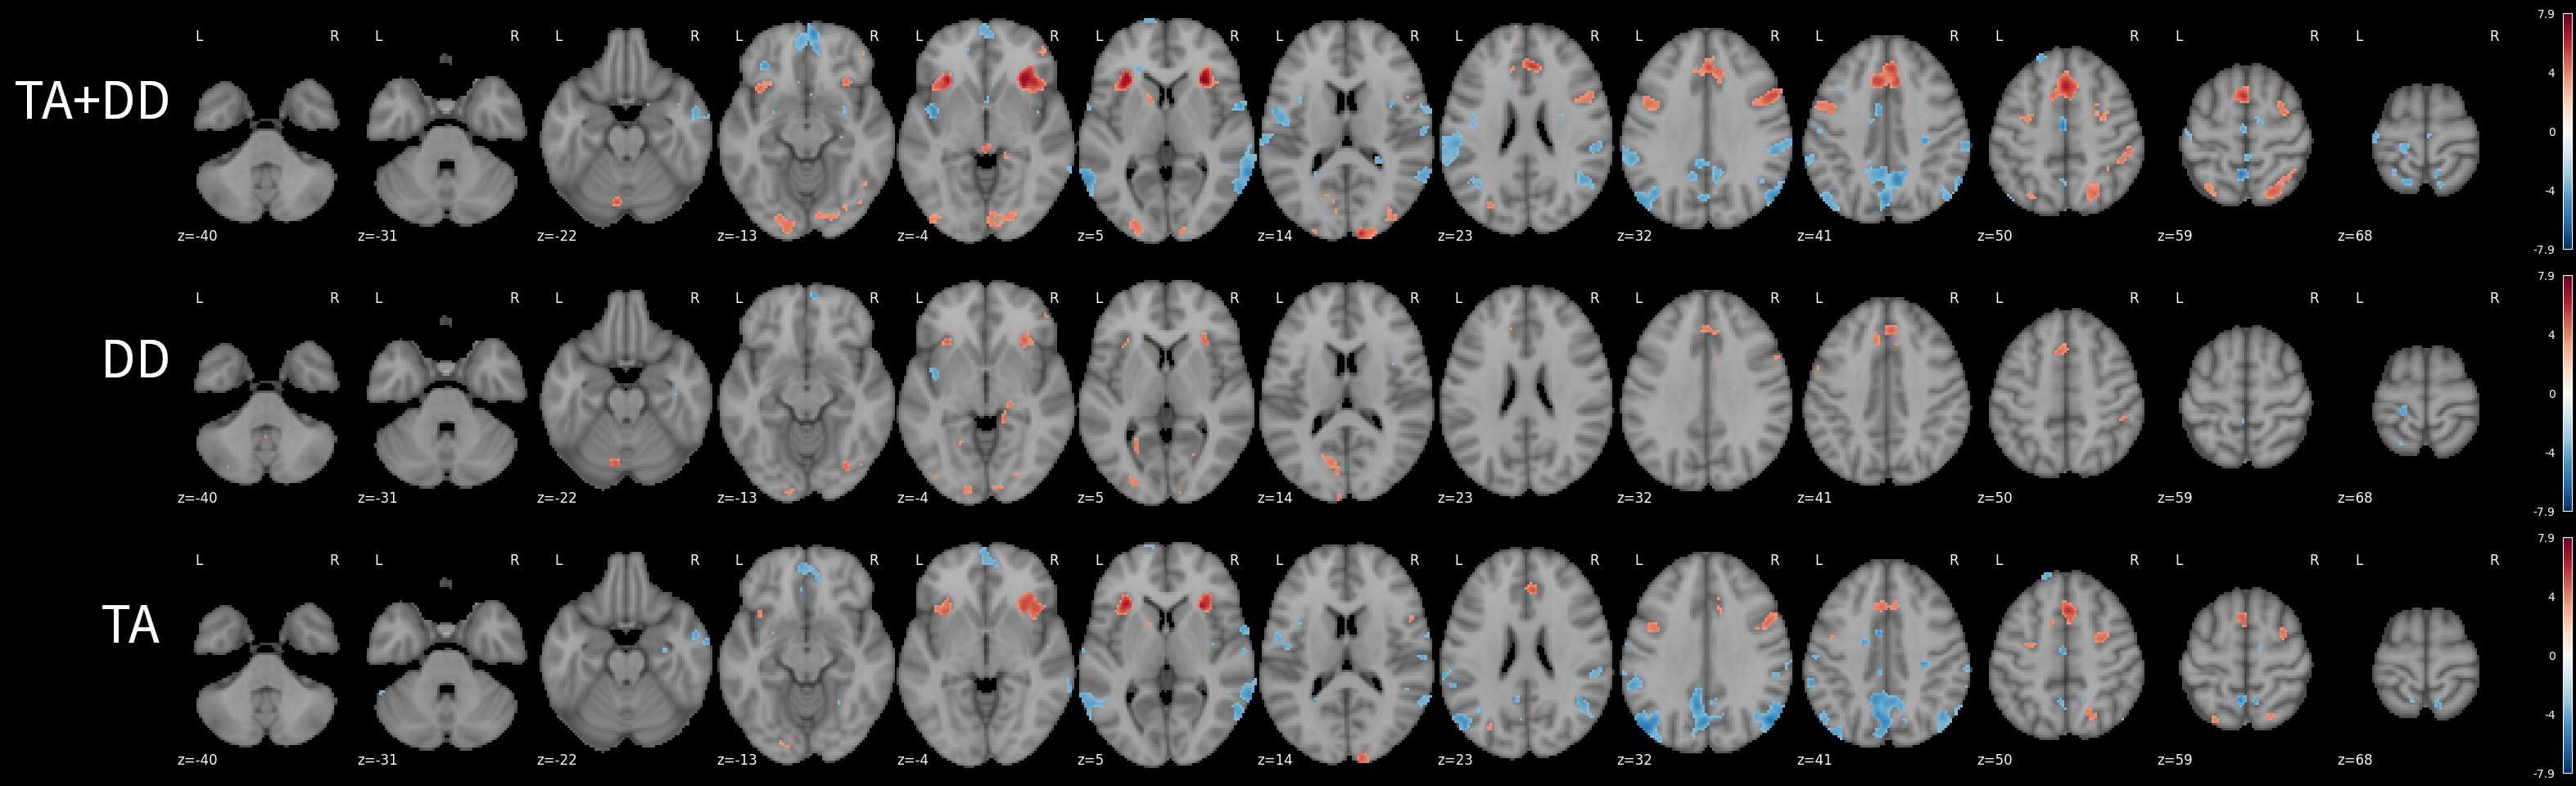
\includegraphics[width=0.95\textwidth]{figures/3_big_small_contrast.png}
	\caption{\label{fig:big_small_contrast} 大小数量对比(c = [-4, -3, -2, -1, 0, 1, 2, 3, 4])在组内的单采样t检测结果($p<0.001$, uncorrected),$-7.9<t<7.9$。从上到下依次为:全体参与者组(DD+TA)、DD组、TA组}
\end{figure}

在两个组中都可以观察到前额叶,前扣带皮质以及前脑岛对于大小数量对比的正响应(对大数有着更高的响应)。有趣的是,在TA组中可以观察到枕叶皮层和后扣带皮层对大小数量对比有着负响应(对大数有着更低的响应),而在DD组中却完全没有此现象。这意味着DD与TA组对于大小数量对比的响应差异也许在枕叶可以得到较好的体现。

\subsection{组间比较}
随后,我们通过基于GLM回归的双采样t检验(对比设计)测试了DD与TA的组间差异。结果如图所示。

\begin{figure}[h]
	\centering
	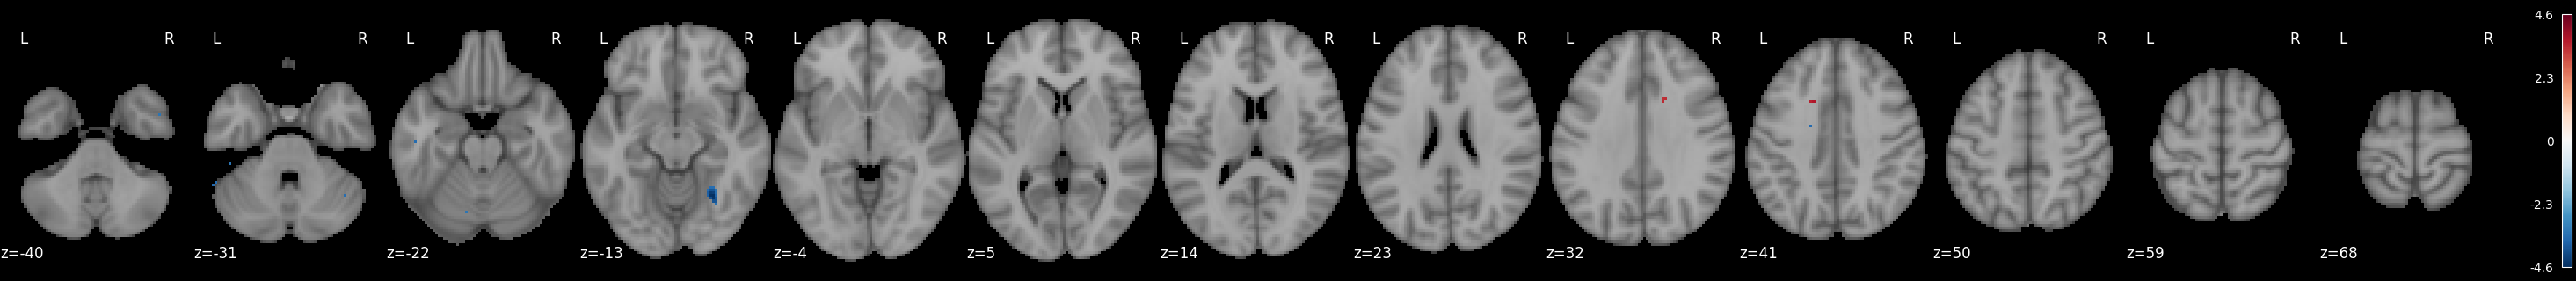
\includegraphics[width=0.95\textwidth]{figures/4_DD_TA_big_small.png}
	\caption{\label{fig:between_group_big_small} 大小数量对比的组间差异($p<0.001$, uncorrected)}
\end{figure}

与预期相悖的是,在枕叶皮层的大部分区域并未观察到显著差异。但是,在右侧视觉腹侧流中有一显著差异区域。为了更好的研究这一差异的显著性,我们进一步设计了多变量的组建分析。

\subsection{基于大小对比的多体素模式分析}
基于以上结论,我们推测数量大小的差异响应是区分DD/TA的神经指标。为了验证此假设,我们使用支持状态机(support vector machine, SVM)分类器进行了多体素模式分析。具体来说,我们将全体对比分成两份:一份用于找出差异响应显著的体素作为遮罩,另一份运用这份遮罩,训练SVM分类器,进行交叉验证(cross validation, CV)。为了保证统计有效性,我们进行10次重复实验,而每次实验的组别区分都来源于随机采样。其中,用于获得遮罩的数据占所有数据的30\%,选择所有$p<0.01$的体素。SVM线性核分类器CV折数为7。最终10次实验的平均CV得分为0.61。

\begin{figure}[h]
	\centering
	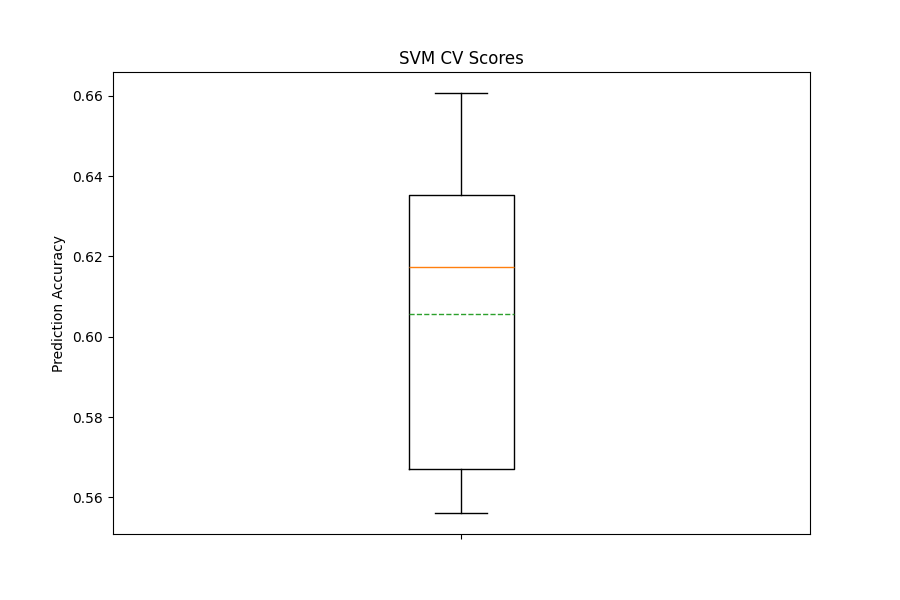
\includegraphics[width=0.60\textwidth]{figures/5_svm_plot.png}
	\caption{\label{fig:svm_plot} 数量大小对比的SVM分类准确性 }
\end{figure}

考虑到将数据集拆分后,每个部分的样本量都较低,无论是特征选择(40个数据点)还是SVM分类器的训练(90个数据点),其数据量都较少。所以,为了确定分类的显著性,我们进行了置换检验(permutation test),其中一次实验的结果如图\ref{fig:6_svm_perm}所示。

\begin{figure}[ht]
	\centering
	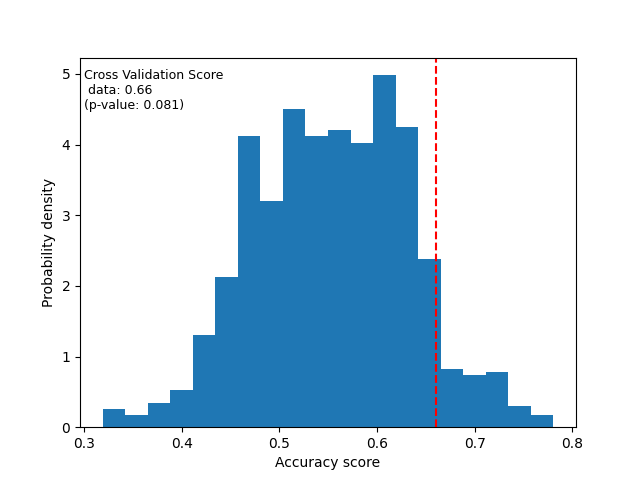
\includegraphics[width=0.60\textwidth]{figures/6_svm_perm.png}
	\caption{\label{fig:6_svm_perm}一次测试的置换检验结果(1000次)。分类的交叉验证得分为0.66($p=0.081$) }
\end{figure}

每次测试的CV得分与置换检验$p$值的关系如表\ref{tab:svm_p}所示。

\begin{table}[htbp]
	\centering
	\begin{tabular}{|c||c|c|c|c|c|c|c|c|c|c|}
		\hline

		\textbf{CV score} & 0.642 & 0.561 & 0.576 & 0.619 & 0.617 & 0.640 & 0.660 & 0.617 & 0.563 & 0.556 \\
		\hline

		\textbf{p value}  & 0.114 & 0.490 & 0.361 & 0.191 & 0.201 & 0.110 & 0.080 & 0.234 & 0.409 & 0.436 \\
		\hline
	\end{tabular}

	\caption{CV得分与置换检验$p$值关系}
	\label{tab:svm_p}
\end{table}

% https://scikit-learn.org/stable/auto_examples/model_selection/plot_permutation_tests_for_classification.html

由此可见,由大小对比的组间差异所确定的特征体素可以用于稳定地区分DD/TA组。但是由于本实验样本量有限,无法得到很强的效应量。

\chapter{讨论} % (fold)
在单个数量刺激的激活图中,我们发现小的数量不会显著激活前额叶,前扣带回,前脑岛皮质。而这些区域与注意力分配,高级认知能力有关\cite{dis1}。这样的现象可能是由于很接近1的数量结构足够简单,以至于小学三年级的孩童无需为其分配过多的注意力。对于较小的数量的认知任务而言,很有可能哪怕对于孩童,该任务也更偏向简单的物体识别任务,而非数量认知任务。而DD、TA人群仅仅在数量1的激活中有显著差异可能意味着DD的神经机理与数作为特殊的基本物体的认知能力有关。

在大小数量对比实验中,我们发现存在对照组孩童的激活比DD组更低的情况。这是原研究未能捕捉到的组间差异。我们猜测,这样的差异来源于DD孩童不能正确地调动学习到的与数量认知特异相关的认知技巧,而还很大程度上依赖于物体识别系统来理解数量。随着数量变大,TA组的响应从视觉相关的通路转换到前额叶皮层,而DD组未能产生与TA组类似的转换。这一猜测也被先前的研究佐证\cite{num19}。

本研究可能存在以下几个问题。一是在数据集的采集中,原作者没有禁止被试通过数数来完成任务。这样可能带来的问题是,更大数量刺激的神经表示中或包含更小数量刺激的神经表示。这会导致小数量刺激的显著性降低。在本研究中所观察到的小数量刺激激活显著少与大数量刺激可能是收到了数数的影响。并且,数数作为另一个数量认知中的重要环节,由于具体的数数情况未知,并无法被建模。这可能会影响模型的准确性,在数据中引入了额外的混淆因素。另一个可能的问题是,本研究将同样数量所对应的阿拉伯数字刺激和点阵刺激归为一类不作区分,但对每个被试的单次试验中,由于变量太多(具体数量,刺激形式,左右刺激),无法排除具体数量模态的影响。在后续研究中可以尝试的做法是将左右刺激以及刺激形式(阿拉伯数字或点阵)都加入到单被试的GLM建模中。这样做可能有助于分离这些因素的影响。

此外,还有一些其他值得后续探索的假设,比如探索韦伯定律在本数据集中的体现以及满足韦伯定律的体素在DD、TA组间的响应差异。本研究碍于时间限制,未能完成的一项分析是在激活簇层面探索与DD、TA差异相关的脑区。这些可能的研究方向都将有助于增进我们对于数量认知以及DD神经机制的理解。


% chapter  (end)

\makebiblio

\begin{acknowledgement}
	在我完成本科生毕业论文的过程中,有许多人的帮助和支持对我至关重要。在此,我谨向所有给予我帮助和支持的人们表达我最诚挚的感谢。

	首先,我要感谢我的导师李远宁老师。在我刚开始这个项目的时候,我并没有完成它所需的知识和远见。在我不断的探索完成此项目的正确的mindset的过程中,是他给予我必要的指引。假如没有他的帮助,完成这个项目是不可能的事情。在最后关头,我真的非常感激他能够包容我的缺点,理解我的处境,并且提供许多极其高效的帮助。这些都是本不可以被期待的事情。同时,我也因为未能更早地以正确的方式和老师合作感到非常可惜。假如我能早些开始以现在的方式推进项目的话,我应该能学到很多很多,也完成更多。

	其次,我要感谢始终陪伴着我的朋友和家人们。是丁涵,王之义,孙静构成了这四年中最最幸福的时光,也是他们在我痛苦地熬夜写论文时给予我支持和陪伴。也特别感谢王之义协助我排版论文,处理图片。

	我还希望感谢在我的成长过程中提供极其宝贵的insight的老师们。感谢李远宁老师带领我进入了计算神经科学的世界,这对我的重要性无需多言。感谢王强老师帮助我重新认识数学,是他让我第一次得以拥有一个人生导师。感谢远在美国的Kevin Andrew Scharp教授告诉我什么是哲学,感谢他欣赏我。非常感谢王之义带着我领会CS的令人窒息的美,没有他耐心,无私的教导,这一切都无法成为可能。事实上,还有很多对我极其重要的老师,但是我无法将他们一一列举,因为我一旦开始尝试列举他们,就有了遗漏的风险。在此,我衷心感谢所有真心教导过我的人。

	最后,我想感谢开源社区的无私奉献。他们所开发的工具和建立的思想给予了我无穷的快乐。仅举几个例子:NixOS社区,Arch Linus社区,Emacs和Doom Emacs社区,Vim和Neovim社区向我展示了一群有着共同爱好的人以一种特殊的,近乎象牙塔的合作方式在一起夜以继日地开发他们所热爱的项目会是多美好的一件事,也向我证明了单纯的热爱就足以驱动许多金钱也难以驱动的事情。这并不是一件平凡的事情。

\end{acknowledgement}

\end{document}
%%% reftex-default-bibliography: ("./reference.bib")
%%% TeX-engine: xetex
